\specialsection{Community}{}{black}{white}

\begin{figure}
	\centering
	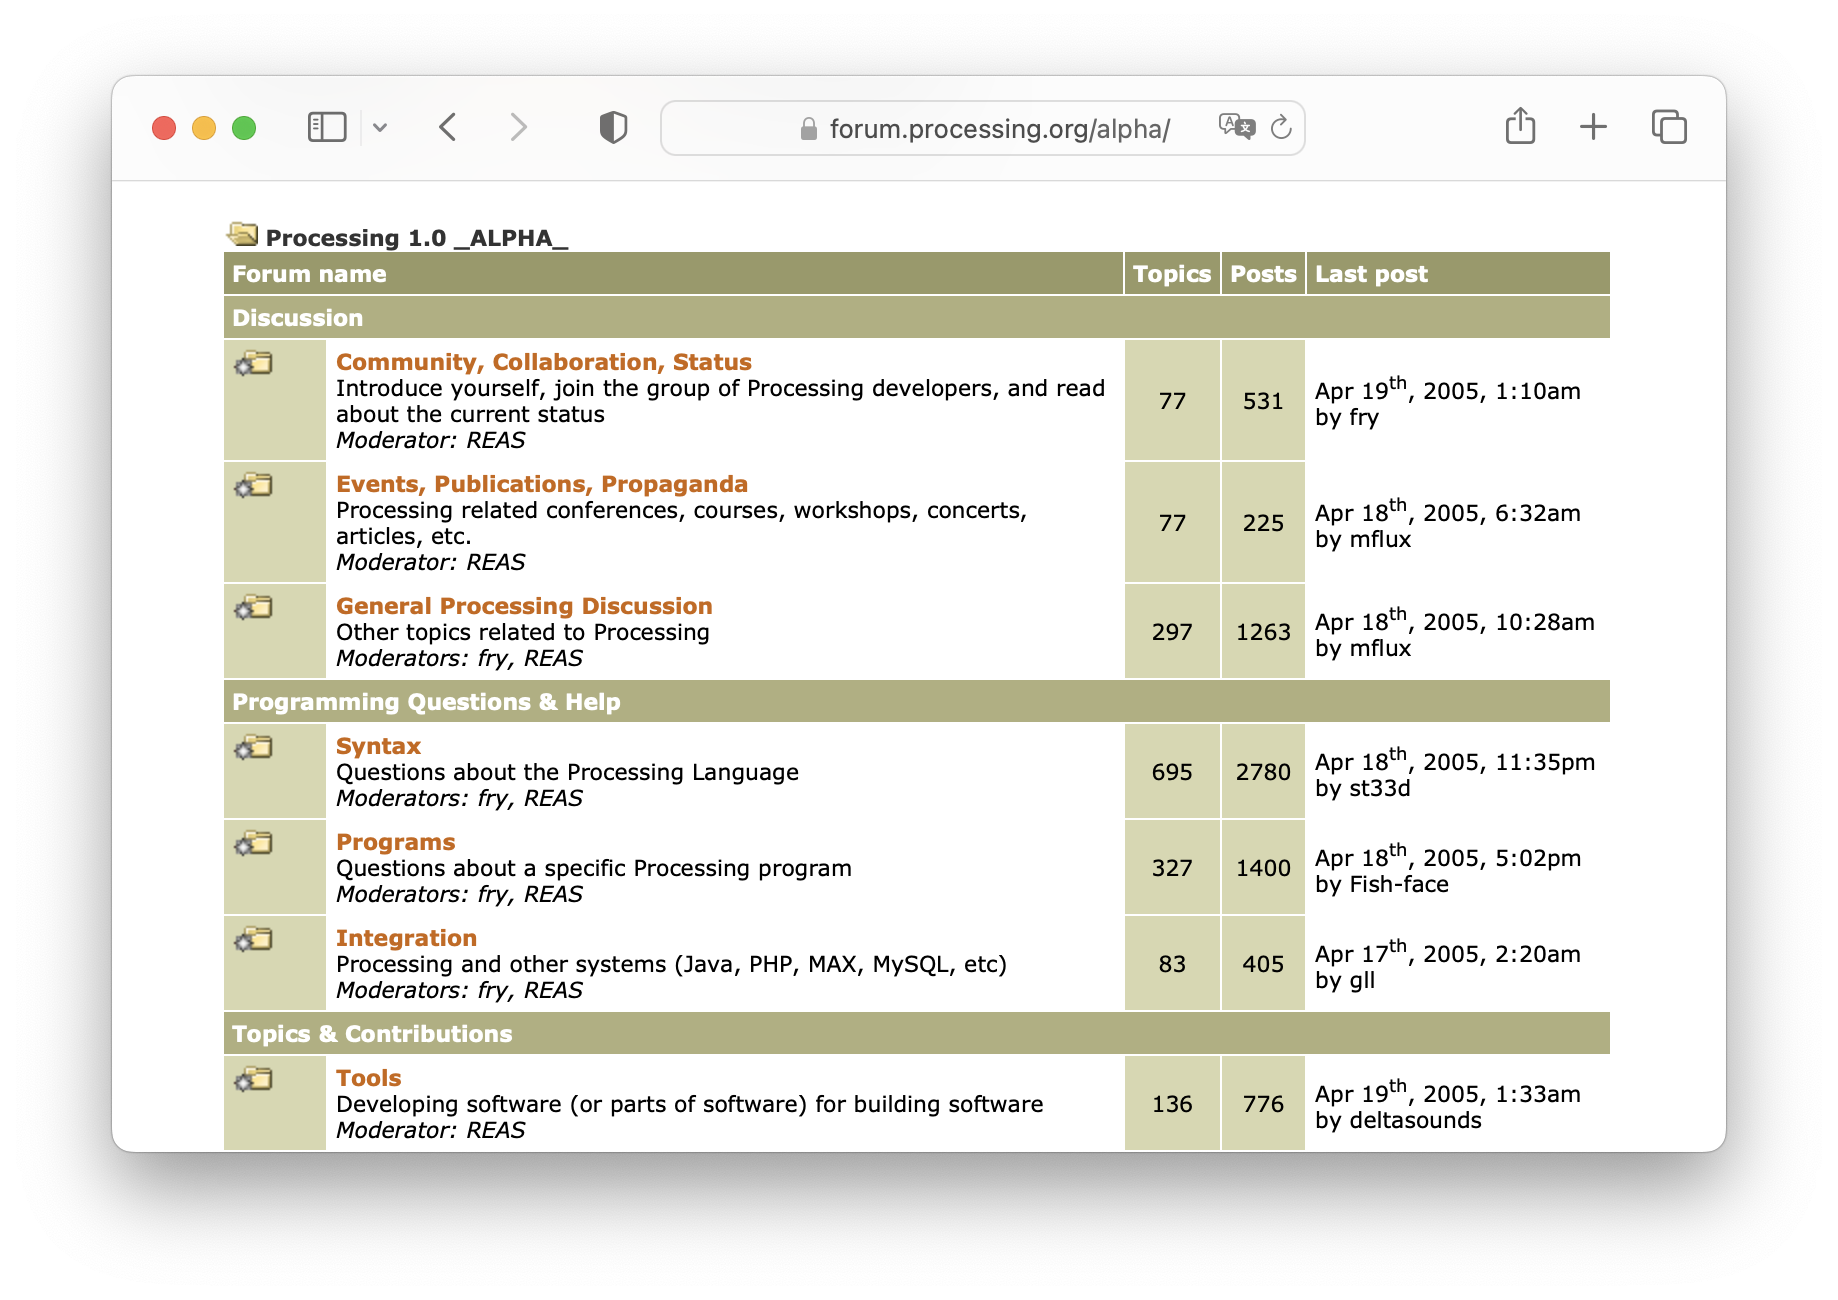
\includegraphics[width=1.0\textwidth]{images/alpha-browser.png}
	\caption{Screenshot of the Processing Alpha Forum}
	\label{fig:processing-alpha}
\end{figure}

\subsection{Community Discussion Platforms}
In the early days of the Processing project, community interactions predominantly took place on forums. These forums, essential for user engagement, evolved in tandem with the versions of the Processing software. Each significant update of Processing was paralleled by a new iteration of the forum, starting from the Processing alpha forum and evolving through beta, 1.0, 2.0 and 3.0 versions, up to the current Processing forum. This progression reflects the software’s development and marks distinct phases in the community's journey. The chronological details of these forum versions, including the years of operation and corresponding URLs, are outlined in Table \ref{table:forums}. \parencite{ProcessingForum}

\begin{table}[h]
	\raggedright
	\begin{adjustbox}{center}
		\begin{tabular}{l l l c}
			\toprule
			Forum name                   & Years      & URL                                                                    \\
			\midrule
			Processing alpha forum       & 2002-2005  & \href{https://forum.processing.org/alpha/}{forum.processing.org/alpha} \\
			Processing beta forum        & 2005-2010  & \href{https://forum.processing.org/beta/}{forum.processing.org/beta}   \\
			Processing 1.0 forum         & 2010-2013  & \href{https://forum.processing.org/one/}{forum.processing.org/one}     \\
			Processing 2.0 and 3.0 forum & 2013-2018  & \href{https://forum.processing.org/two/}{forum.processing.org/two}     \\
			Current processing forum     & 2018 - now & \href{https://discourse.processing.org/}{discourse.processing.org}     \\
			\bottomrule
		\end{tabular}
	\end{adjustbox}
	\caption{Archival forums composition}
	\label{table:forums}
\end{table}

% Choice and importance of the alpha forum
The Alpha forum was subjected to data scraping and a preliminary analysis. This process was instrumental in identifying active members for potential interviews. The forum’s significance, as underscored by Reas, was a key consideration in this analysis. Reas asserted that the forum cultivated a ‘unified international community’ from 2002 to 2006 \parencite[331]{conradGraphicDesignPostdigital2021}, further highlighting its importance. This exploration provides valuable insights into the early stages of the Processing project and its community dynamics.

% Interviews
In the exploration of online communities within the realm of computational design, the study focused on key members of the Alpha forum, namely Ariel Malka (arielm), Martin Gomez (Martin), and Jacob Schwartz (benelek). These individuals were selected for their active participation in the forum, without holding additional roles such as library contributors. Their diverse geographic and academic backgrounds, alongside their forum experiences, illuminate the role of online platforms for individuals when real-life peer networks in specialized fields are absent or limited.

Ariel Malka (arielm), influenced by his father, an artist painter, and his early interest in graphic design and programming, found a significant community within the Alpha forum. His involvement in the forum was pivotal, especially considering the lack of a similar interest group in his immediate environment. He articulated this connection, saying, "finalement, ouais j'ai beaucoup participé et euh même un peu trop. Des fois je racontais ma vie carrément. Mais euh, c'était un besoin apparemment"​​. This highlights the forum's role as his primary platform for engaging with computational design, particularly in architectural applications.

Martin Gomez (Martin), during his college years studying computer science and information systems, experienced isolation in his home country regarding computational design. He transitioned from traditional design to using Processing and contributing to its development. His engagement with the forum was necessitated by the absence of a local community with similar interests, as he observed, "There weren't really anyone apart from me doing this in, in, in my country at the time"​​.

Jacob Schwartz (benelek), with interests spanning generative art, programming, art, and architecture, but without a formal background in computing, found the forum invaluable. The forum served as both a learning environment and a source of inspiration. He gained significantly from sharing his work and receiving feedback, as well as from observing the professional applications of other members. Schwartz reflected on this, stating, "I got a lot out of posting what I was working on and then getting feedback from that and also looking at what other people were working on and seeing how they did those things"​​.

In conclusion, the involvement of Ariel Malka (arielm), Martin Gomez (Martin), and Jacob Schwartz (benelek) in the Alpha forum illustrates its critical role as a platform for engagement, learning, and inspiration in computational design. This is particularly evident in their cases, where their unique geographic and academic backgrounds contributed to a lack of similar interests in their immediate physical and academic environments. The forum not only bridged this gap but also fostered a sense of community and growth in their respective fields of interest.

% Library and code contributors
The academic and professional environments of library contributors like Ricard Marxer, Andreas Schlegel, and Simon Greenwold in the Processing community indeed present a stark contrast to the experiences of those primarily active in forums, such as Ariel Malka (arielm) and Jacob Schwartz (benelek).

Ricard Marxer's discovery of Processing during his master's studies in digital art around 2004-2005, set in a context that bridged programming and digital art, fostered an ideal environment for his library development. Unlike forum-centric users, Marxer's engagement with the Processing community was marked more by his technical contributions than by active forum participation. His self-taught background in computing and his focus on maintaining his library between 2002-2010, as opposed to seeking peer interaction on forums, underscores a different path within the community​​​​.

Similarly, Andreas Schlegel created the OSC P5 library as part of his final year project, reflecting a more academic-driven involvement. Schlegel's work on this library, stemming from his educational pursuits, highlights a focus on project-specific needs over community engagement in forums​​.

Complementing this, Simon Greenwold's contributions to Processing were significantly shaped by his academic and teaching roles. His time at the MIT Media Lab, interacting with the Aesthetics and Computation Group under John Maeda and corresponding with Processing's co-founders, Ben Fry and Casey Reas, provided a rich backdrop for his technical development. Greenwold worked on core aspects like the camera and lights in Processing and developed a particle system physics library, primarily for teaching purposes. His approach to the Processing community was less about forum participation and more focused on the technical and educational aspects, aligning with his background at institutions like Harvard and his lack of substantial engagement in online forums and communities​​​​.

In essence, Marxer, Schlegel, and Greenwold's deep-rooted academic and professional settings shaped their contributions to Processing differently than forum-centric members like Malka and Schwartz. These contributors were less reliant on the Processing forums for community support and interaction, focusing more on leveraging Processing in their academic and teaching activities. This delineation highlights the diverse motivations and environments influencing the engagements and contributions within the Processing community, ranging from community-driven interaction to academic and technical innovation.

% graph of the alpha forum contributors
\changepapersize{305.3mm:210mm}
\customtag{largepage}

{
	\LARGE
	\noindent Alpha Forum Top Contributors\par
	\vspace{0.2cm} 
}
\vfill

\begin{figure}[h!]
	\centering
	\frame{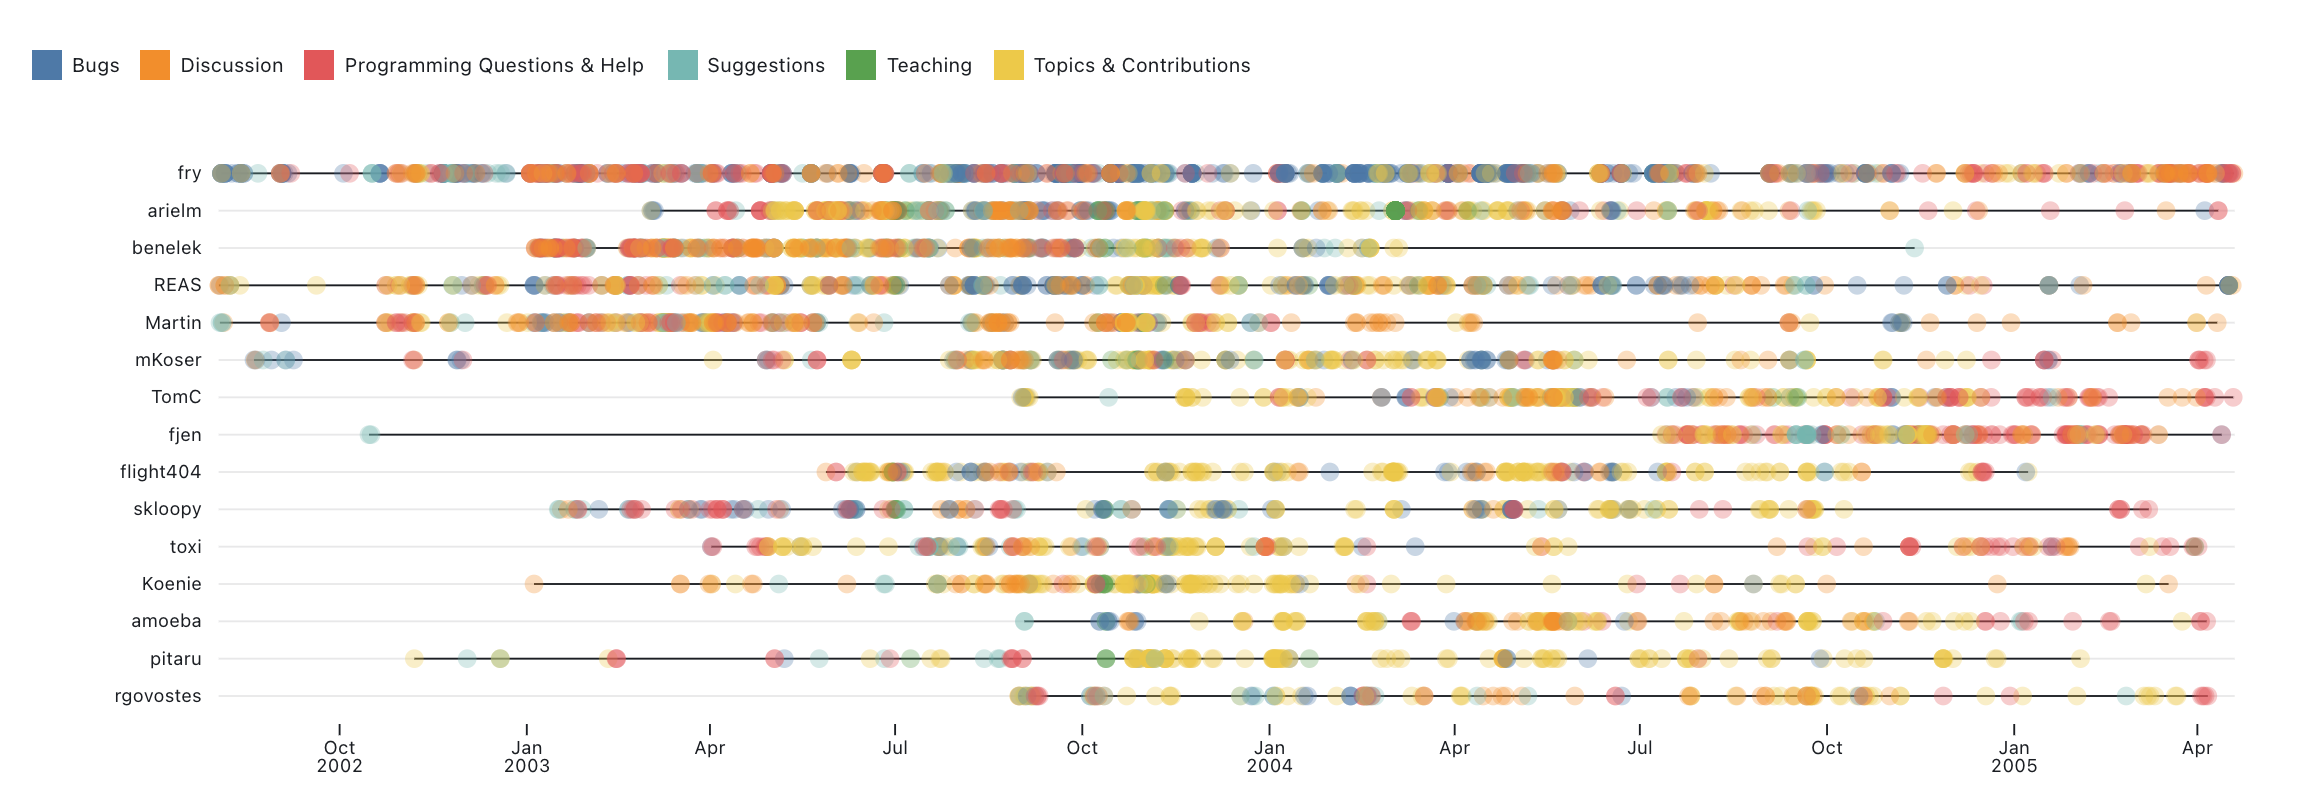
\includegraphics[width=1.0\textwidth]{images/alpha-forum-top15.png}}
	\caption{Posting activity of the 15 most active contributors on the alpha forum.}
	\label{fig:processing-alpha-dot}
\end{figure}

% Add commentary to the graph
\begin{multicols}{3}
	\noindent
  Figure \ref*{fig:processing-alpha-dot} shows a timeline of color coded post by category of the 15 most active contributors to the Alpha forum. Among them Ariel Malka (arielm), Jacok Schwartz (benelek) and Martin Gomez (Martin) were interviewed, on the basis of their participation in the forums, with no definitive indications of them assuming additional roles such as library contributor. We can observe certain patterns emerging such as initial posts being often in the Programing Help \& Questions section, often spanning out to others in the future. A part from co-creators Ben Fry (fry) and Casey Reas (REAS) we can also observe clustering of posts for users, suggesting periods of activity and inactivity. 
  \columnbreak

  \vfill\null
  % \parbox{\linewidth}{}
  % \eject
\end{multicols}
\defaultareasettings

% TODO - important ingredients in community success

Ben Fry is the most active forum contributor, but the activity distribution is more balanced than in Git commits, possibly due to the diverse topics covered, including technical queries and bugs. A total of 1,039 individuals contributed to the forum discussions as shown in Figure~\ref{fig:processing-alpha-dot}.
Linus's Law—"Given enough eyeballs, all bugs are shallow" \parencite[29]{raymondCathedralBazaar1999}—is somewhat evidenced by increased forum activity during release periods, suggesting community involvement in bug identification, as demonstrated in Figure~\ref{figure:forum-git-activity}.

\begin{figure}[!htbp] 
    \centering 
    %\includesvg[pretex=\sffamily\fontsize{5.58pt}{8pt}\selectfont, width=1\textwidth, keepaspectratio]{images/figure-forum-git-activity.png}
    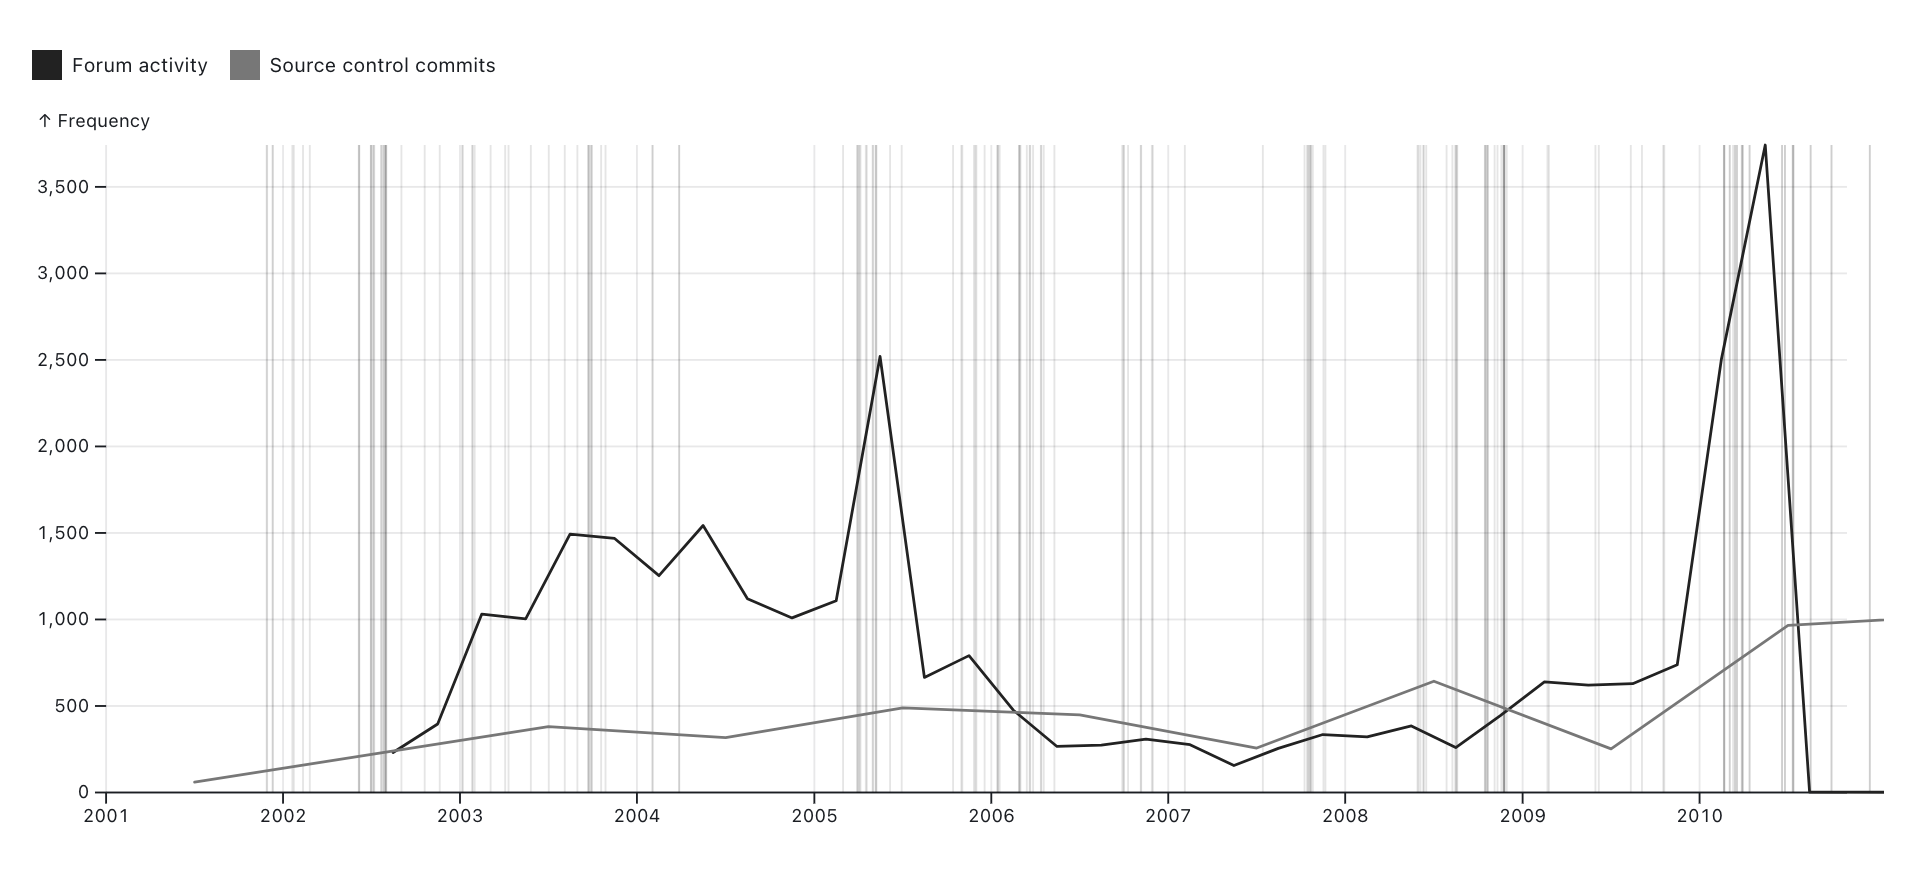
\includegraphics[width=1\textwidth]{images/figure-forum-git-activity.png} 

    \caption{Forum vs git activity vs releases (vertical lines)}
    \label{figure:forum-git-activity}  
  \end{figure}

Contrary to the initial assumption that primary contributors would predominantly be from the MIT ACG group, given the project's origins, a preliminary analysis suggests otherwise.

\begin{figure}[htbp]
	\centering

	% Row 1
	\begin{subfigure}[b]{0.24\textwidth}
		\includesvg[pretex=\sffamily\fontsize{5.58pt}{8pt}\selectfont, width=1\textwidth, keepaspectratio]{images/month1.svg}
		\caption{Month 1}
		\label{fig:month1}
	\end{subfigure}
	\hfill
	\begin{subfigure}[b]{0.24\textwidth}
		\includesvg[pretex=\sffamily\fontsize{5.58pt}{8pt}\selectfont, width=1\textwidth, keepaspectratio]{images/month2.svg}
		\caption{Month 2}
		\label{fig:month2}
	\end{subfigure}
	\hfill
	\begin{subfigure}[b]{0.24\textwidth}
		\includesvg[pretex=\sffamily\fontsize{5.58pt}{8pt}\selectfont, width=1\textwidth, keepaspectratio]{images/month3.svg}
		\caption{Month 3}
		\label{fig:month3}
	\end{subfigure}
	\hfill
	\begin{subfigure}[b]{0.24\textwidth}
		\includesvg[pretex=\sffamily\fontsize{5.58pt}{8pt}\selectfont, width=1\textwidth, keepaspectratio]{images/month4.svg}
		\caption{Month 4}
		\label{fig:month4}
	\end{subfigure}

	% Add space between rows
	\vspace{0.25cm}

	% Row 2
	\begin{subfigure}[b]{0.24\textwidth}
		\includesvg[pretex=\sffamily\fontsize{5.58pt}{8pt}\selectfont, width=1\textwidth, keepaspectratio]{images/month5.svg}
		\caption{Month 5}
		\label{fig:month5}
	\end{subfigure}
	\hfill
	\begin{subfigure}[b]{0.24\textwidth}
		\includesvg[pretex=\sffamily\fontsize{5.58pt}{8pt}\selectfont, width=1\textwidth, keepaspectratio]{images/month6.svg}
		\caption{Month 6}
		\label{fig:month6}
	\end{subfigure}
	\hfill
	\begin{subfigure}[b]{0.24\textwidth}
		\includesvg[pretex=\sffamily\fontsize{5.58pt}{8pt}\selectfont, width=1\textwidth, keepaspectratio]{images/month7.svg}
		\caption{Month 7}
		\label{fig:month 7}
	\end{subfigure}
	\hfill
	\begin{subfigure}[b]{0.24\textwidth}
		\includesvg[pretex=\sffamily\fontsize{5.58pt}{8pt}\selectfont, width=1\textwidth, keepaspectratio]{images/month8.svg}
		\caption{Month 8}
		\label{fig:month 8}
	\end{subfigure}

	% Add space between rows
	\vspace{0.25cm}

	% Row 3
	\begin{subfigure}[b]{0.24\textwidth}
		\includesvg[pretex=\sffamily\fontsize{5.58pt}{8pt}\selectfont, width=1\textwidth, keepaspectratio]{images/month9.svg}
		\caption{Month 9}
		\label{fig:month9}
	\end{subfigure}
	\hfill
	\begin{subfigure}[b]{0.24\textwidth}
		\includesvg[pretex=\sffamily\fontsize{5.58pt}{8pt}\selectfont, width=1\textwidth, keepaspectratio]{images/month10.svg}
		\caption{Month 10}
		\label{fig:month10}
	\end{subfigure}
	\hfill
	\begin{subfigure}[b]{0.24\textwidth}
		\includesvg[pretex=\sffamily\fontsize{5.58pt}{8pt}\selectfont, width=1\textwidth, keepaspectratio]{images/month11.svg}
		\caption{Month 11}
		\label{fig:month11}
	\end{subfigure}
	\hfill
	\begin{subfigure}[b]{0.24\textwidth}
		\includesvg[pretex=\sffamily\fontsize{5.58pt}{8pt}\selectfont, width=1\textwidth, keepaspectratio]{images/month12.svg}
		\caption{Month 12}
		\label{fig:month12}
	\end{subfigure}

	\caption{Monthly graphs}
	\label{fig:monthlyGraphs}
\end{figure}


\begin{figure}[h!]
	\centering
	\includesvg[pretex=\sffamily\fontsize{5.58pt}{8pt}\selectfont, width=1\textwidth, keepaspectratio]{images/year.svg}
	\caption{Year}
	\label{figure:year}
\end{figure}


%\begin{figure}[h!] 
    \centering 
    \includesvg[pretex=\sffamily\fontsize{5.58pt}{8pt}\selectfont, width=1\textwidth, keepaspectratio]{images/figure-forum-posts.svg}
    \caption{Top 12 authors by number of posts (Aggregated alpha and beta forum)}
    \label{fig:forum-posts}  
  \end{figure}

%\begin{figure}[htbp] 
    \centering
    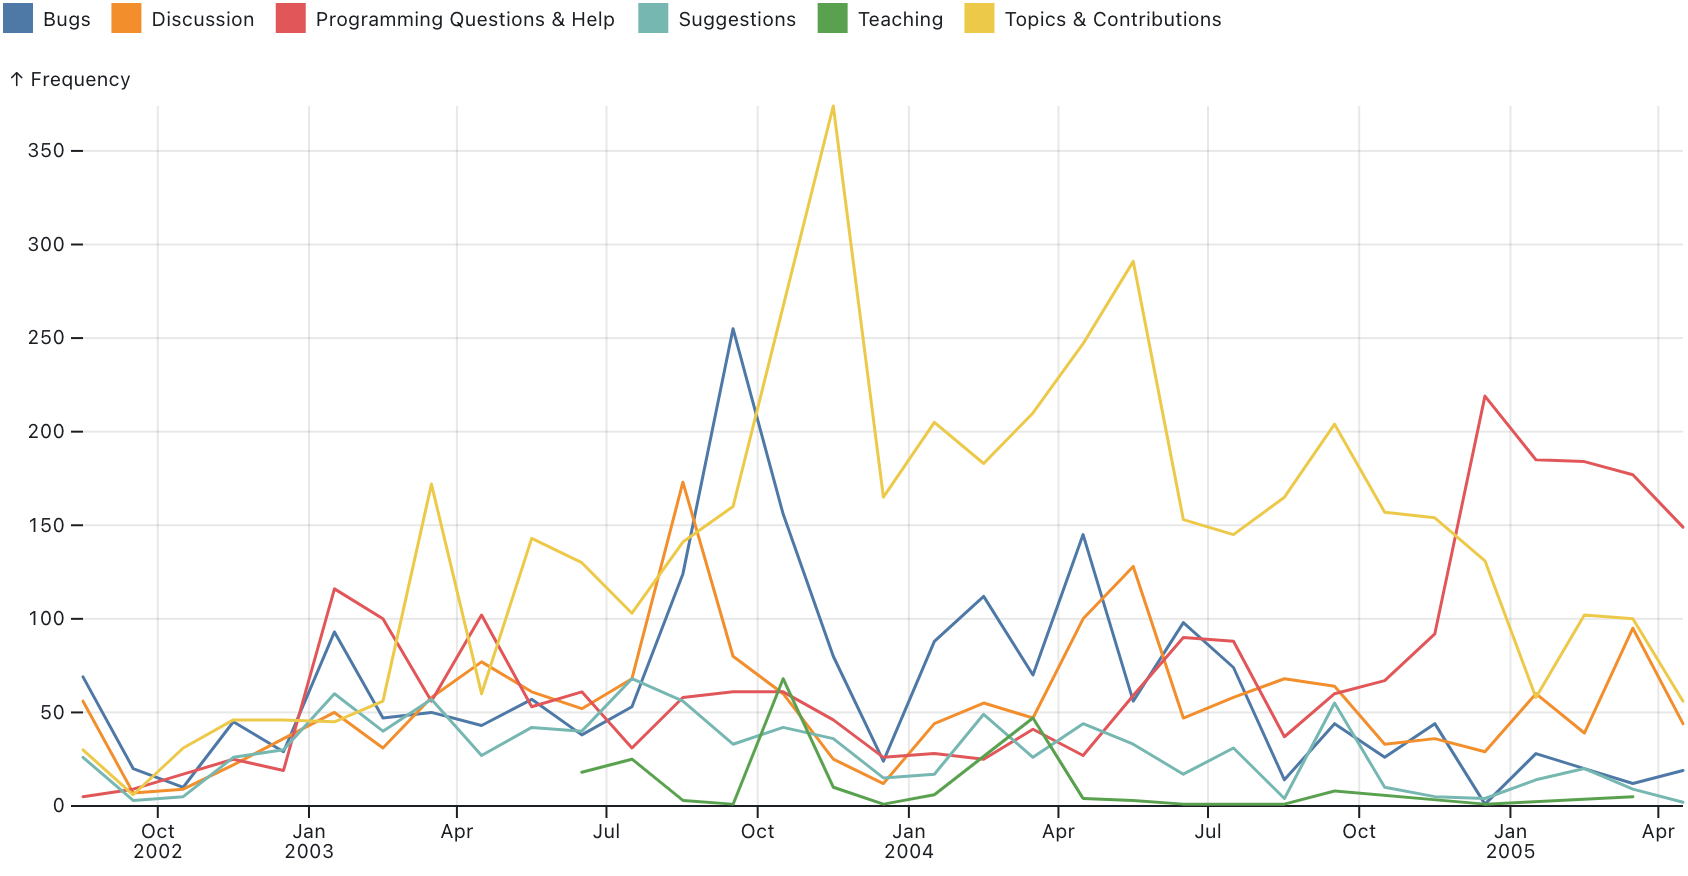
\includegraphics[width=1\textwidth]{alpha-forums-activity.png} 
    % \includesvg[pretex=\sffamily\fontsize{5.58pt}{8pt}\selectfont, width=0.6\textwidth]{images/alpha-forums-activity.svg}
    \caption{Forums activity}
    \label{fig:forum-activity}  
  \end{figure}

%\begin{figure}[h!] 
    \centering 
    \includesvg[pretex=\sffamily\fontsize{5.58pt}{8pt}\selectfont, width=1\textwidth, keepaspectratio]{images/figure-alltime-sourcecode-commits.svg}
    \caption{Top 25 source code contributors by number of commits}
    \label{fig:alltime-sourcecode-commits}  
  \end{figure}

%\begin{figure}[htbp] 
    \centering
    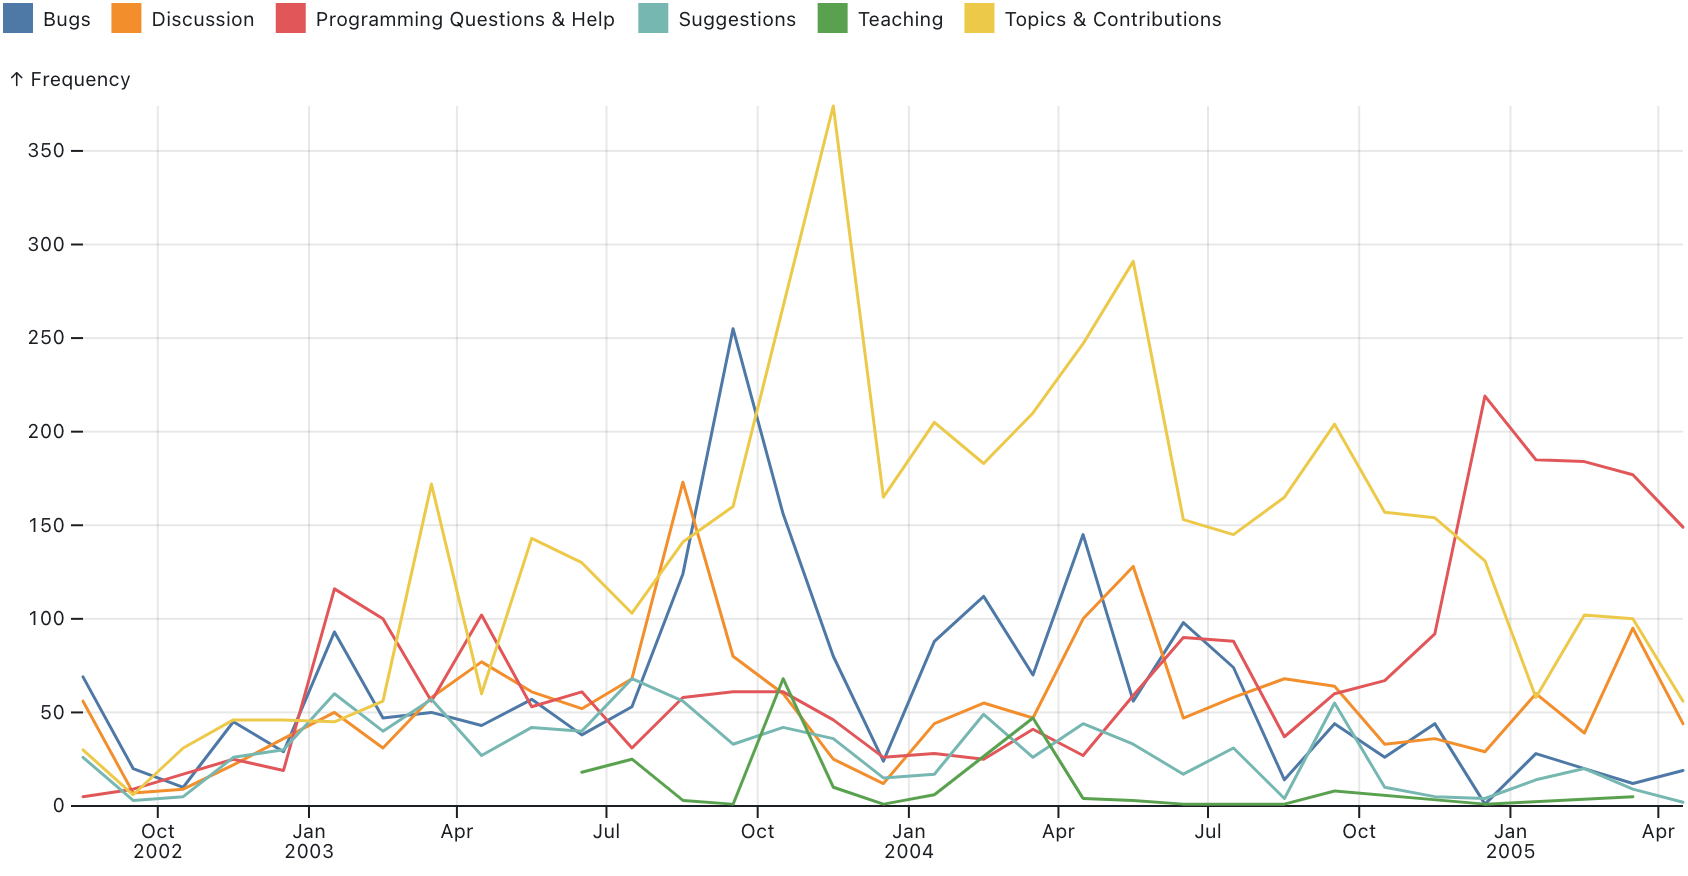
\includegraphics[width=1\textwidth]{alpha-forums-activity.png} 
    % \includesvg[pretex=\sffamily\fontsize{5.58pt}{8pt}\selectfont, width=0.6\textwidth]{images/alpha-forums-activity.svg}
    \caption{Forums activity}
    \label{fig:forum-activity}  
  \end{figure}

% \subsubsection{Synthesized Data Analysis: Git Commits, Releases, and Forum Activity}

% \subsubsection{Alpha Forum Patterns in Forum Contributions (to remove)}
There were 11,926 posts across 2,626 topics from 02/08/2002, 15:29 to the 19/04/2005, 09:55 across 1039 authors in the forum.

The alpha forum was a YaBB (Yet another Bulletin Board), it was seperated into forums which conained boards which contained topics which contained posts.

\begin{figure}
    \centering 
    \includesvg[pretex=\sffamily\fontsize{5.58pt}{8pt}\selectfont, width=1\textwidth, keepaspectratio]{images/alpha-forums-by-posts.svg}
    \caption{Topics by post number}
    \label{fig:forums}  
  \end{figure}


\subsection{A culture of workshops}

\begin{figure}[h]
	\centering
	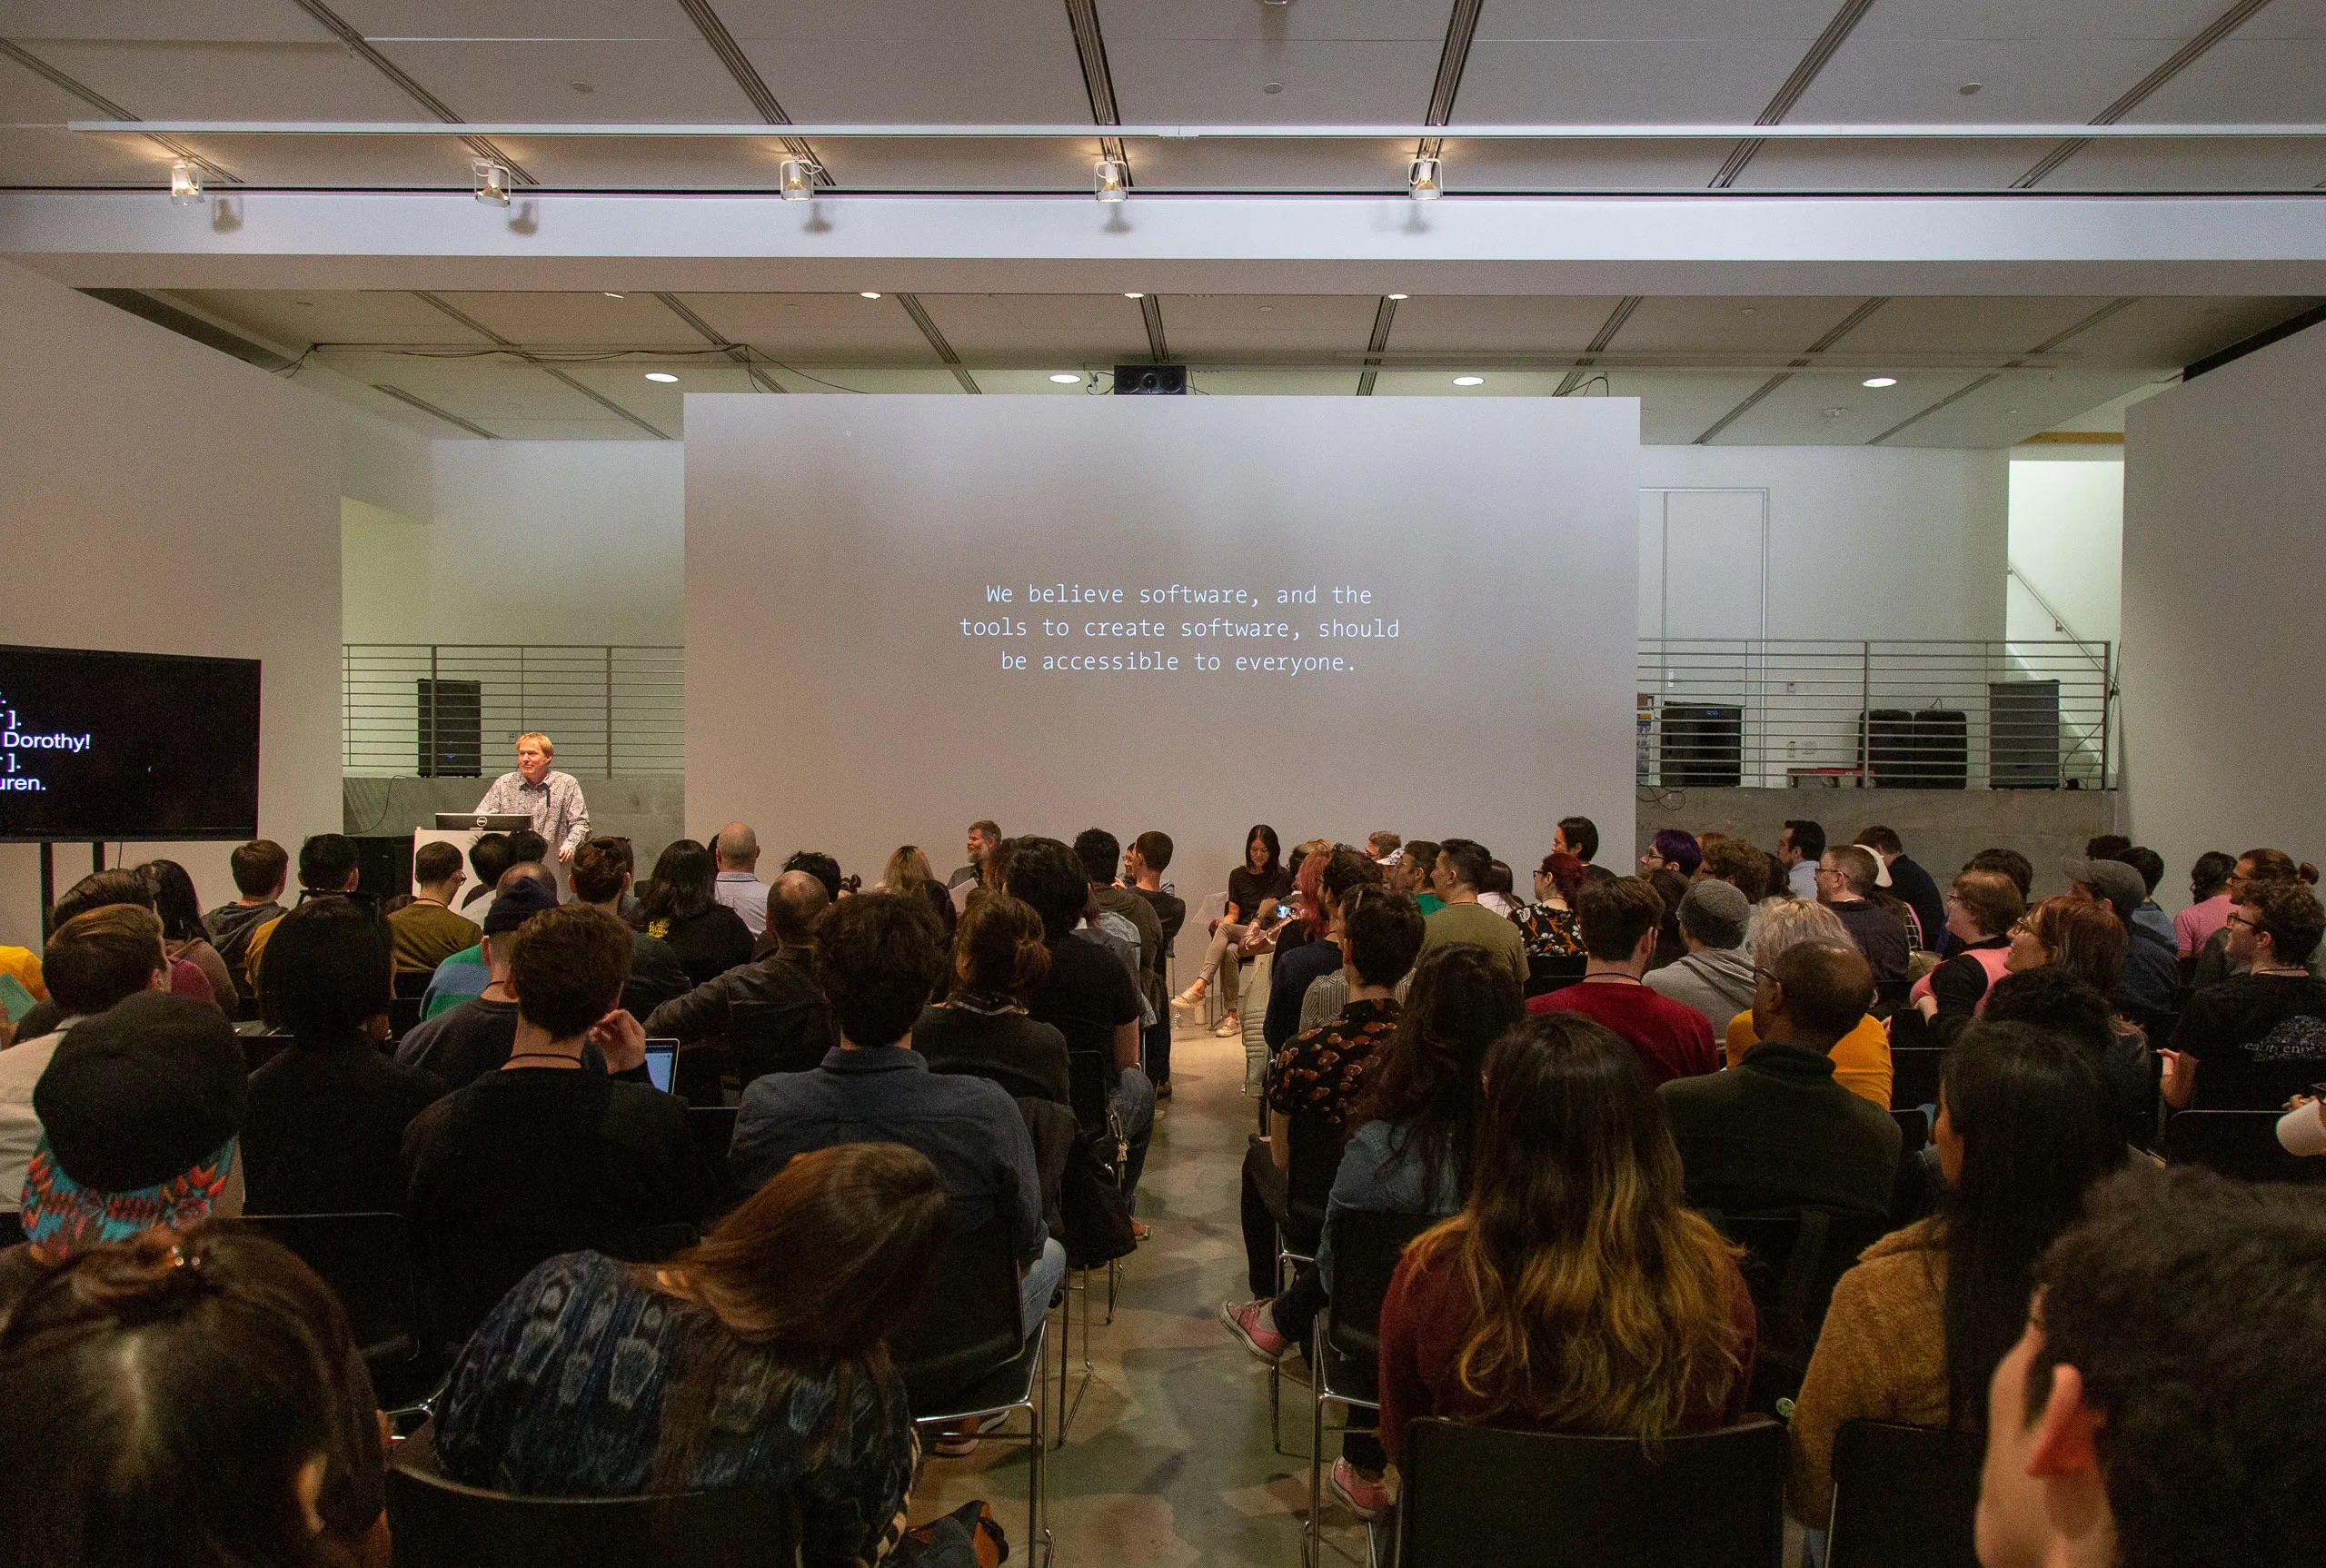
\includegraphics[width=1\textwidth]{images/pcd_la_2019.jpeg}
	\caption[Ben Fry at PCD 2018]{Ben Fry with conference attendees. Source: \citefield{guptaBenFryConference2018}{author}, Medium, \citeyear{guptaBenFryConference2018}.}
\end{figure}

\subsection{An ecosytem of libraries}
An important milestone in the Processing ecosystem was the introduction of libraries. These libraries extended the functionalities of the base platform, thereby attracting a broader range of users and contributors. Such an analysis not only sheds light on the diversification of the project but also identifies key contributors and library authors who could potentially be sought out for qualitative interviews. The identification of these contributors adds another layer to our understanding of community participation.

\changepapersize{305.3mm:210mm}
\customtag{largepage}

\begin{figure}
	\includesvg[pretex=\sffamily\fontsize{5.58pt}{8pt}\selectfont, width=1\textwidth, keepaspectratio]{images/figure-libraries.svg}
	\caption{Distribution of Libraries in the Processing Project}
	\label{figure:libraries}
\end{figure}

\defaultareasettings

\subsection{Processing Foundation}

The Processing Foundation was established in 2012 by Casey Reas, Ben Fry, and Daniel Shiffman with the primary objective of sustaining the software's development and broadening its reach. According to Fry and Reas, ``The vast majority of the code is written by the same small number of people volunteering their time — there are no paid full-time developers'' \parencite[p.~13]{fryModernPrometheusHistory2018}.

\begin{figure}[h]
	\centering
	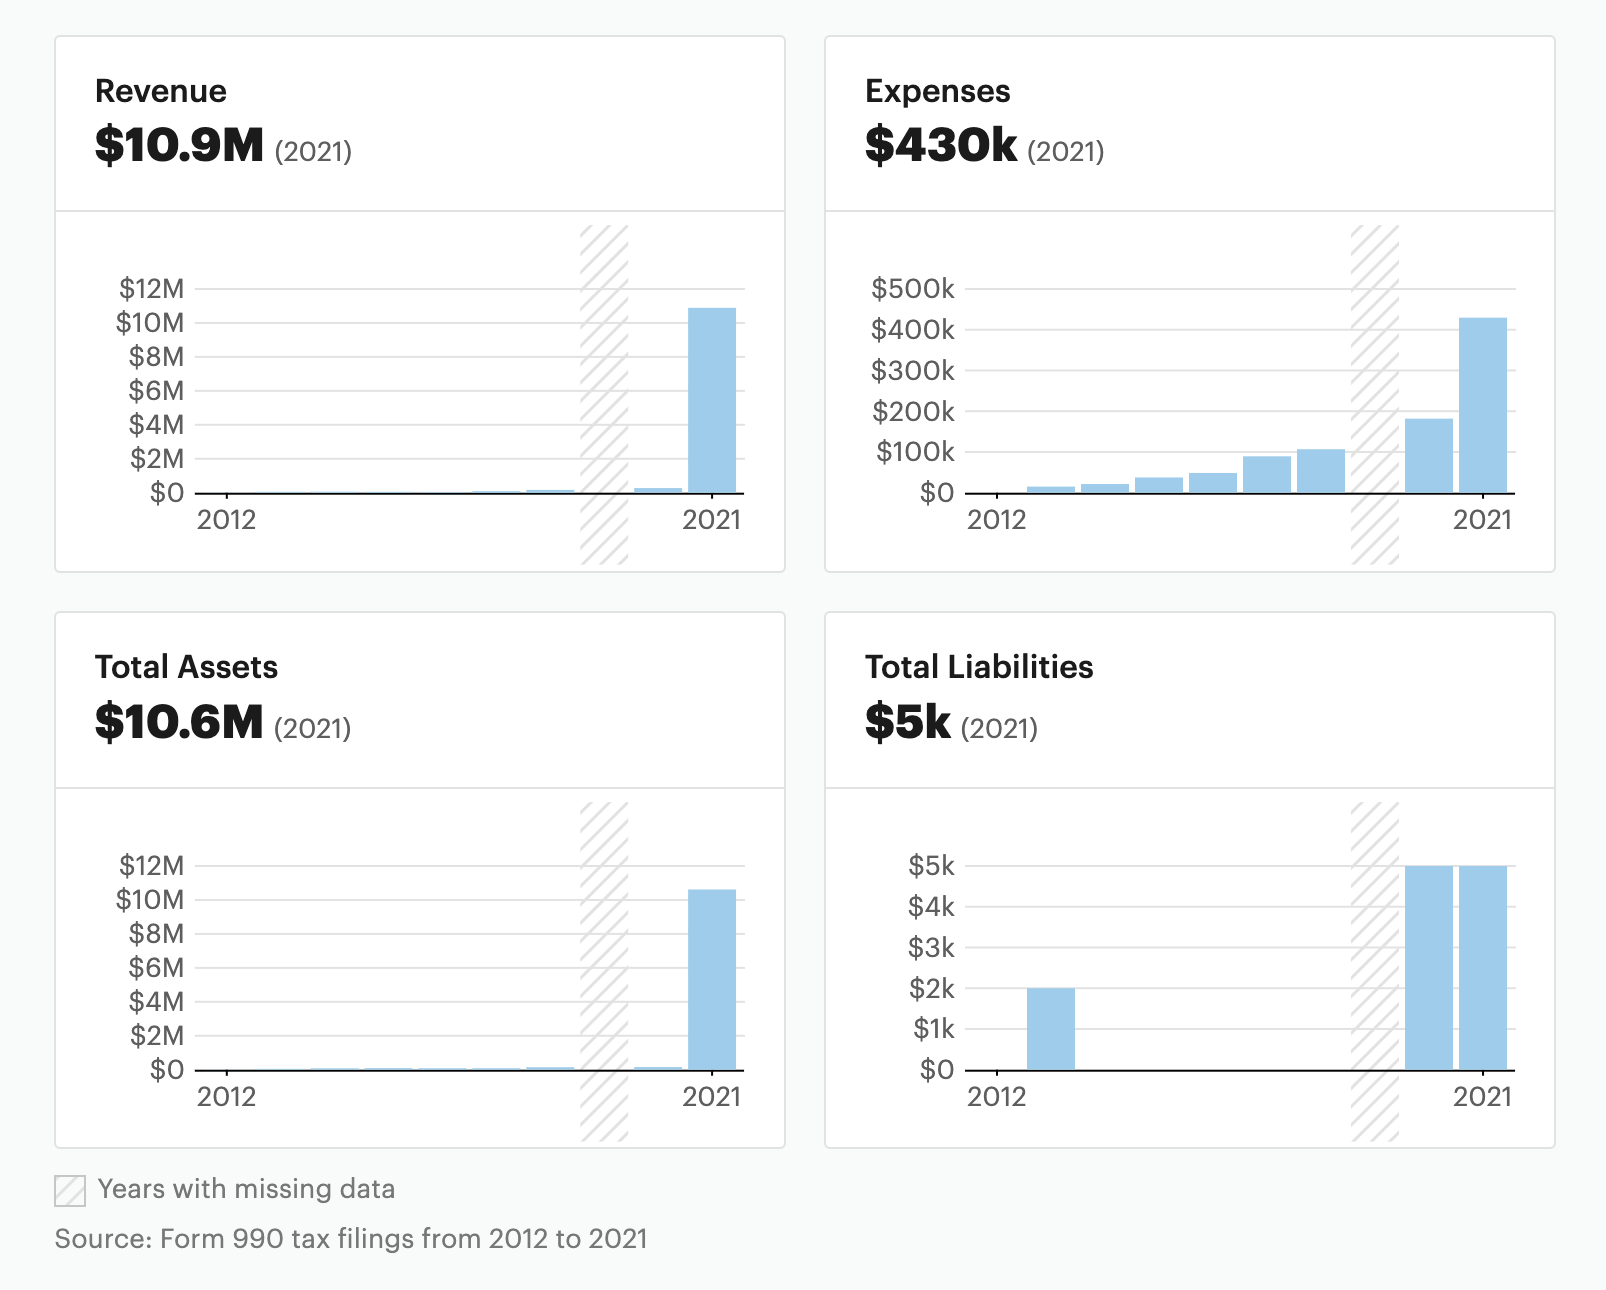
\includegraphics[width=0.9\textwidth]{images/foundation-finances.png}
	\caption{Financial growth of the Processing Foundation over the years Source: \parencite{ProcessingFoundationNonprofit2013}}
	\label{fig:foundation-finances}
\end{figure}

As shown in Figure~\ref{fig:foundation-finances}, the foundation's revenue has experienced modest growth, increasing from \$11,235 to \$273,520. Remarkably, it reached a peak revenue of \$10,889,998 in the fiscal year 2021. Throughout its history, the principal source of funding for the foundation has predominantly come from contributions.

However, the allocation of these funds has been a point of contention within the organization. Most notably, a public disagreement in 2023 led to the resignation of Ben Fry, a long-standing board member and contributor. It should be noted that Fry's perspective on the matter was not universally accepted among the foundation's other founding members. \parencite{benfry[@ben_fry]HaveMadeExtremely2023} \parencite{caseyreas[@reas]EarlierThisWeek2023} \parencite{danielshiffman[@shiffman]WouldPostNote2023}

